\chapter{Configuration and Testing}
\label{configurationandtesting}
This chapter will contain the configuration of all nodes of the concept. In addition the newly developed nodes have to be tested as well as the entire navigation concept.


The structure of this chapter is to address the outer nodes of the navigation concept first and then move to the inner nodes.\\


\section{URDF and Robot State Publisher}

\section{Gazebo}

\subsection{Plugins}

\section{Filter}

\subsection{road\_detection}

\subsection{laser\_filter}

\subsection{robot\_localization}

\subsection{markfreespace}

\section{Cartographer}

\section{PoseFinder}
\section{Planners}
\section{Costmaps}
Based on the fact that both planners are responsible for different tasks the configuration of the individual costmaps need to fulfill different tasks too. Here we can compare the requirements of the two planners, from which we can determine how the costmaps will be defined.\\

As described in the theoretical knowledge of this thesis the costmap are structured in layers. This means that the data can be evaluated by different plugins before it will be combined into the real costmap.\\

It makes sense to first take a look at the general behaviour, that both planners share. In this case it is obstacle avoidance. This means that the lethal obstacles need to be marked in both costmaps.\\

To realize this the provided plugin obstacle\_layer can be used. It will take incoming sensor data (sensor\_msgs::PointCloud or sensor\_msgs::LaserScan) and mark the points in the costmap.\\

Since the data here comes form the road detection and a lidar and both have a certain resolution it is unsure, if the result of a scanned obstacle in the costmap is actually a closed line or just points, since this highly relies on the resolution of the sensors and the costmap.\\

To fill theses gaps in the costmap the provided plugin inflation\_layer can be used. It will inflate only the lethal obstacles in the costmap with a configurable cost distribution.\\

This setup is already enough for the local costmap, where as the global planner needs to fulfill the quest of changing lanes if necessary but all-ways preferring the right lane. For this a custom plugin will be needed that makes the transition to the left lane more expensive but still possible.

\subsection{dynamic\_cost\_layer}
Enhancing to the plugins provided in the navigation stack this layer handles inflation of cells with a configurable cost decay and radius. While this seems to be similar to the provided inflation layer, this offers way more flexibility since it will inflate specific points by their individual radius and cost distribution and not just every lethal one by one fixed distribution.\\

This behavior can be used to inflate the left road marking in the global costmap to force the global plan on the right side of the road. The plugin can also be used to inflate cells with zero cost, which is useful to guarantee a cost free right lane or to give some free space around obstacles located on the road.\\

The layer receives a message of type sensor\_msgs::PointCloud on a configurable topic. This PointCloud is expected to feature Channel Values for the inflation radius, the maximal and the minimal cost for each individual point.\\

Since we can't assume that the incoming points will be in the frame of the costmap the points in the costmap have to be transformed into the right frame using tf2.\\

To minimize the computation load a bresenham based algorithm for the circle rasterization will be used. Now the point symmetry around the cell can be used to further minimize the computational load and only $\frac{1}{8}$th of the circle has to be computed. The rasterization process can be described by the following image.\\

Adding to the typical behavior of the bresenham rasterization the area of the circle will be filled with the cost specified for the point. For this the following linear decaying \nth{1} degree function will be used which requires the computation of the distance of the rasterized cell to the center of the circle.

\[cost(distance)=maxcost-distance*\frac{maxcost-mincost}{radius}\]\\
with: \[distance=\sqrt{cell.x^2+cell.y^2}\]

 Since this will still require the usage of a square root for each cell in the circle This will be optimized as well.\\

The goal here is to use a function that contains only the squared distance, which still represents a decaying trend. This requirement rules out every function with an odd degree, as well as all functions with an x offset. This leaves all functions with an even degree from which we choose the \nth{2} degree function to reduce square operators. The comparison between the two functions can be seen in the picture below.

\[cost(distance)=maxcost-distance^2*\frac{maxcost-mincost}{radius^2}\]\\
\begin{figure}[h!]
	\begin{center}
	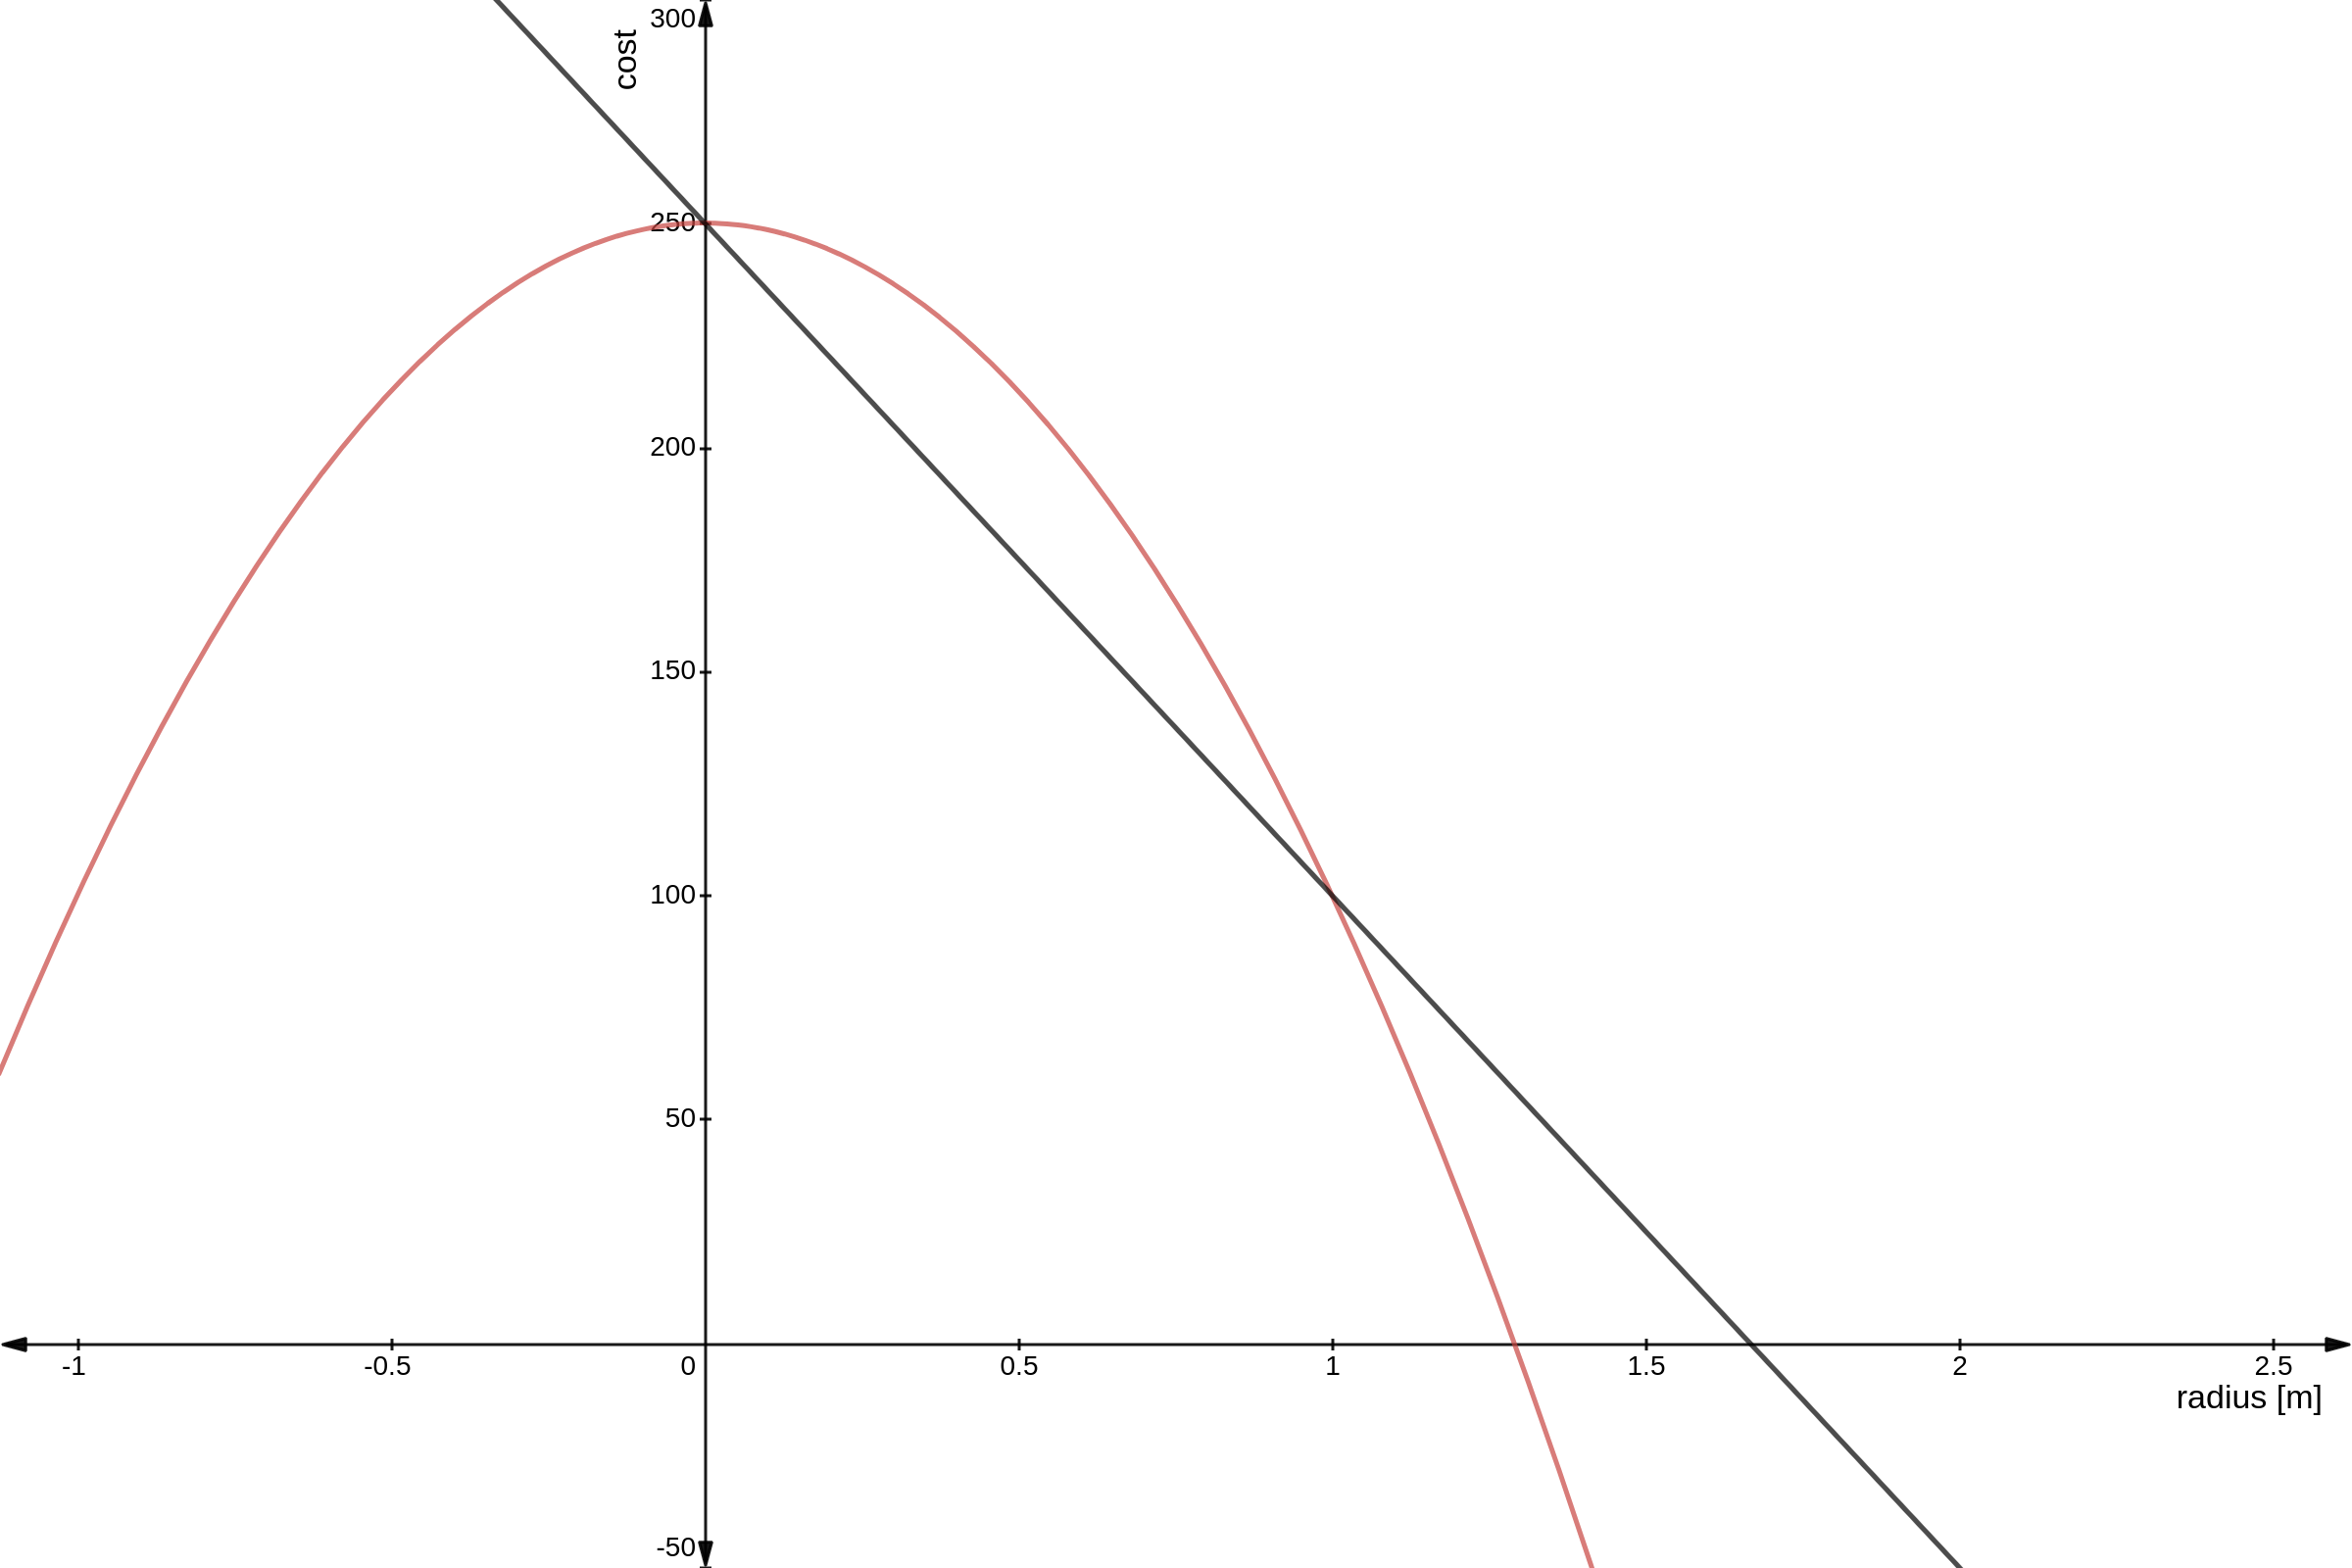
\includegraphics[width=140mm]{Pictures/linear cost comparison}
	\caption{cost distribution comparison with maxcost=250 mincost=100 radius=1}
\end{center}
\end{figure}



\subsection{global\_costmap}

\subsection{local\_costmap}
\subsection{global\_planner}
\subsection{local\_planner}

